\chapter{Auswertung Benchmark}
Im folgenden werden die Ergebnisse des Benchmarks ausgewertet.
Dazu wird zu erst die Gesamtlaufzeit des Benchmarks in \autoref{auswertung:generell} analysiert. Dabei wird zwischen zeilenbasierten und spatenbasierten
Tabellen unterschieden.
Anschließend wird in \autoref{auswertung:queries} auf die Laufzeit der
einzelnen Unterabfragen des Benchmarks eingegangen.
Dabei soll untersucht werden welche Abfragen besonders schnell sind.
In \autoref{auswertung:basic_indizes} und \autoref{auswertung:hardware}
wird der Einfluss von Indizes bzw.\ unterschiedlicher Hardwarekonfigurationen
untersucht.

\section{Gesamtlaufzeit des Benchmarks}\label{auswertung:generell}

\begin{tabularx}{\textwidth}{|X|r|r|}
	\toprule
	 & \textbf{Rowstore} & \textbf{Columnstore}\\
	\midrule
	\endhead
	\hline
	\caption{Gesamtlaufzeiten von Row- und Columnstore in usec}
	\label{auswertung:gesamtlaufzeit}
	\endfoot
	Durchschnitt & 754689 & 3591003 \\
	Minimum & 725710 & 3451791 \\
	Maximum & 858595 & 4079505 \\
	Median & 752236 & 3577376 \\
	Standardabweichung & 17619 & 79002\\
	Gesamt & 754689 & 3591003 \\
\end{tabularx}

Allgemein sollten Benchmarks auf der HANA Datenbank immer zwischen
Row- und Columnstore unterscheiden.
Dies wird deutlich beim Betrachten der Allgemeinen Laufzeit.
Wie \autoref{auswertung:gesamtlaufzeit} zu entnehmen ist, besteht ein deutlicher
Unterschied in der Laufzeit zwischen Row- und Columnstore.
Da der SSBM Benchmark als Maß für Abfragen im Bereich des Datawarehouse
eingesetzt wird, kann also allgemein gesagt werden,  dass der Columnstore
dem Rowstore im Datawarehouse Umfeld vorzuziehen ist.
Jedoch sollte bedacht werden, dass es sich bei dem SSBM Benchmark um
reine Abfragen von Daten handelt. Wie in \autoref{row_col:rowstore} beschrieben
kann ein Rowstore von Vorteil sein, wenn Daten gespeichert werden.

\begin{figure}[H]
	\centering
	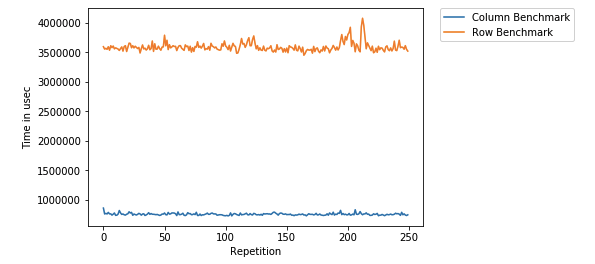
\includegraphics[width=0.7\textwidth]{images/performanceentwicklung.png}
	\caption{Gesamtlaufzeit von Row- und Columnstore}\label{auswertung:gesamtlaufzeit:graph}
\end{figure}
Anhand der Standardabweichung und \autoref{auswertung:gesamtlaufzeit:graph} ist auch zu sehen, dass der Columnstore
eine konstantere Zeit pro Abfrage aufweist.
Allerdings da der Rowstore im allgemeinen langsamer ist als der Columnstore
kann dies vernachlässigt werden, da die Standardabweichung relativ zur
Gesamtlaufzeit sehr gering ist.

\section{Vergleich der SSBM Queries}\label{auswertung:queries}

Im folgenden werden die einzelnen Queries des SSBM Benchmarks separat betrachtet.

%TODO
% Vergleich von q1, q2, q3, q4 etc.
% Diagramm
% Welche ist die schnellste und warum?
% Stabilität einzelner Queries

\newpage
\section{Einfluss der grundlegenden Indizes}\label{auswertung:basic_indizes}
Die Benchmarkergebnisse in diesem Abschnitt wurden auf folgender Hardware erzielt:
\begin{itemize}
    \item Host: i7 7700k, 16GB DDR4 RAM
    \item VM: 6 Kerne @90\%, 8GB RAM
\end{itemize}
%TODO
% Row with or without indices
% Column with or without indices

\subsection{Grundlegende Untersuchung für Column-Store}

\begin{table}[H]
\centering
    \begin{tabularx}{10cm}{lrrr}
        \toprule
        Merkmal             &   Col[ms]    &    Col Index[ms] & Abweichung[\%]\\
        \toprule
        Samples             &   250        &   250      &        \\
        \midrule    
        Max                 &   859        &   697      & -18.8\%\\
        Min                 &   726        &   546      & -24.7\%\\
        Median              &   752        &   574      & -23.6\%\\
        Average             &   755        &   578      & -23.4\%\\
        Standard Deviation  &   18         &   19       & +5.5\%\\
        Total               &   188672     &   144605   & -23.3\%\\
        \bottomrule
    \end{tabularx}
\caption{Vergleich der Ergebnisse mit und ohne grundlegende Indizes für Column-Store.}
\label{tab:basic_index_col}
\end{table}

Durch hinzufügen der grundlegenden Indizes wurde der Benchmark
für Columstores sowohl im Schnitt als auch im Median schneller.
Im Schnitt wurde er 23,4\%, im Median um 23,6\% schneller.
Die Standardabweichung hat sich jedoch nur geringfügig verändert.
Die Werte streuen relativ gesehen also gleich stark wie zuvor.
Folglich konnten Mindest- und Maximallaufzeit auch deutlich reduziert werden. 


Diese Ergebnisse sind interessant,
da Columnstores bereits einen natürlichen Index
durch speichern der Daten in Spalten haben,
wie in \autoref{sec:col_store} beschrieben.
Deshalb profitieren Columnstore meist nicht von zusätzlichen Indizes.
Um herauszufinden, warum trotzdem eine deutliche Verbesserung merkbar ist,
wird der Query-Execution Plan des Subqueries mit der deutlichsten Verbesserung
im folgenden untersucht.

\subsubsection{Untersuchung der Laufzeit für einzelne Query-Gruppen}

\begin{table}[H]
    \centering
    \begin{tabularx}{14cm}{lrrr}
        \toprule
        Benchmarkgruppe & Col[ms]   & Col Index[ms] & Laufzeitreduzierung[ms|\%]\\
        \toprule
        Q1              & 104.7       & 68.5            & 36.2 | 34.5\%\\
        Q2              & 62.1        & 59.7            & 2.4 |  03.8\%\\
        Q3              & 96.2        & 54.8            & 41.4 | 40.8\%\\
        Q4              & 112.4       & 106.3           & 6.1 |  05.4\%\\
        \bottomrule
    \end{tabularx}
	\caption{Durchschnittslaufzeit für jede Benchmarkgruppe für Column-Store.}
\end{table}

Deutliche Verbesserungungen sind bei den Queries der Gruppen 1 und 3 festzustellen. Hier hat sich die Laufzeit um 35\% bzw. sogar 41\% reduziert. 
Die Queries dieser Gruppe werden im Detail untersucht, um geeignete Kandidaten für die Analyse des Execution-Plans zu finden.
Hier sind besonders bei Query 1.2 und 3.4 interessant, da diese die größte Verbesserung in ihrer Gruppe vorweisen können. 
Die Laufzeit wurde um 64\% für Query 1.1 und um mehr als 90\% für Query 3.4 reduziert. Woher diese Verbesserung kommen, soll im Folgenden durch die Analyse der Execution-Pläne von Query 1.1 und 3.4 geklärt werden.


\begin{table}[H]
    \centering
    \begin{tabularx}{13cm}{lrrr}
        \toprule
        Benchmark           & Col[ms]       & Col Index[ms] & Laufzeitreduzierung[ms|\%]   \\
        \toprule
        Q1.1                & 36.1          & 36.4          & -0.3 | -0.8\%                \\
        Q1.2                & 47.8          & 16.8          & 31.0 | 64.8\%                 \\
        Q1.3                & 21.3          & 14.1          & 7.2 | 33.8\%                \\
        Q3.1                & 31.3          & 31.6          & -0.3 | -0.9\%                \\
        Q3.2                & 24.0          & 18.9          & 5.1 | 21.2\%                 \\
        Q3.3                & 21.3          & 2.1           & 19.2 | 90.1\%                \\
        Q3.4                & 20.5          & 1.6           & 18.9 | 92.1\%                \\
        \bottomrule
    \end{tabularx}
\caption{Durchschnittslaufzeit für Benchmarkgruppe 3 für Column-Store.}
\end{table}

\subsubsection{Analyse des Query-Execution-Plans für Query 3.4}

Bei der Analyse des Query-Execution Plans zeigt sich schnell,
woher die große Geschwindigkeitssteigerung kommt.
In Query 3.4 bildet einen Join von Lineorder auf Customer,
Supplier und Dim\_Date. 
Dieser Join erfolgt jeweils über den Fremdschlüssel in Lineorder.
Ohne Indizes ist dieser Join ausschlaggebend für die Laufzeit des Querys.
Durch anlegen von Indizes auf alle Fremdschlüssel,
kann der Join deutlich schneller ausgeführt werden.
Den größten Vorteil hat hier der Index auf LO\_Suppkey.

Der Execution Plan ohne Indizes ist in \autoref{execution-plan:before-index}
zu finden und der Execution Plan mit Indizes ist in \autoref{execution-plan:after-index} zu finden.

Query 3.1 im Vergleich nutzt zwar auch Fremdschlüssel, um einen Join zu bilden,
allerdings sind hier die nicht indizierten Felder \verb+S_Region+, \verb+D_Year+,
\verb+C_Nation+ und \verb+S_Nation+ in der Where- und der Group by-Klausel gelistet,
wodurch eine Geschwindigkeitsverbesserung nicht möglich ist.

Auch bei Column-Stores scheinen sinnvoll angelegte Indizes also einen deutlichen Unterschied zu machen.

\subsubsection{Analyse des Query-Execution-Plans für Query 1.2}
%https://archive.sap.com/discussions/thread/3429357
Bei Query 1.2 gibt es eine Besonderheit: Manchmal wird der Query über die OLAP-Engine ausgeführt\footnote{Um zu sehen, welche Engine verwendet wird, muss anstatt \enquote{Visualize Plan} die Option \enquote{Explain Plan} gewählt werden.}. 
Hierbei ist der Laufzeitunterschied zwischen Index und kein Index fast nicht mehr vorhanden, der Query mit Index braucht allerdings weniger Zeit zur Kompilation. 
Eigentlich ist die OLAP-Engine für \enquote{Analytical Views}, die im Star-Schema vorliegen gedacht, was beim Star-Schema Benchmark ja definitv der Fall ist.
Allerdings ist nicht klar, warum die OLAP-Engine manchmal verwendet wird und manchmal nicht. Ein Muster war hier nicht zu erkennen. 


%http://saphanatutorial.com/sap-hana-modeling/
%https://archive.sap.com/discussions/thread/3340726
Zunächst trat die OLAP-Engine nur auf, wenn Indizes hinzugefügt wurden, weshalb zunächst angenommen wurde, dass HANA an Hand der Indizes erkennt, dass es sich im Grunde um einen Analytical View handelt und dementsprechend optimiert.
Allerdings gab es auch Fälle, wo die OLAP-Engine auch ohne Indizes verwendet wurde. Kommt die OLAP-Engine zum Einsatz, so ist der Query deutlich schneller. Die folgenden Zahlen sind leider nur Ergebnisse einzelner Durchläufe, 
da den Benchmark \enquote{repräsentativ} oft auszuführen und paralell festzuhalten, welcher Durchlauf mit welcher Engine durchgeführt wurde, hier leider den Rahmen sprengen würde.

Kommt nicht die OLAP-Engine, sondern die \enquote{normale} Column-Engine zum Einsatz, so gibt es einen deutlichen Unterschied zwischen Index und kein Index. Hierbei kann der Index auf LO\_OrderDateKey für den JOIN genutzt werden und beschleunigt diesen somit.
Außerdem wird die Berechnung \textbf{sum(lo\_extendedprice*lo\_discount)} deutlich beschleunigt. Warum ist allerdings nicht klar, denn auf diese Felder wurde kein Index angelegt.

An dieser Stelle unterscheidet sich der Execution-Plan nur in diesem Wert:
\begin{description}
    \item[Kein Index] <executePop(<lockInputs(num=3,)=0.00><calculateOnAttr(<calculateWithAggregation(rows=4301,inputs=2,outputs=1,)=8.04>rows=4301,outputs=1,)=8.15>)=11.61>
    \item[Index]      <executePop(<lockInputs(num=3,)=0.00><calculateOnAttr(<calculateWithAggregation(rows=4301,inputs=2,outputs=1,)=1.03>rows=4301,outputs=1,)=1.10>)=1.18>
\end{description}

Die letzte Zahl scheint jeweils die Laufzeit in ms zu sein, aber eine genaue Erklärung dieser Werte war leider nicht zu finden.

\begin{table}[H]
    \centering
    \begin{tabularx}{14cm}{lXX}
        \toprule
        Engine              & Col (Comp | Exec)[ms]                 & Col Index (Comp | Exec)[ms]     \\
        \toprule
        OLAP                & 7.18 | 10.04          & 0.13  | 10.29         \\
        Colum               & 7.64 | 40.85          & 11.44 | 17.90          \\   
        \bottomrule
    \end{tabularx}
	\caption{Durchschnittslaufzeit für jede Benchmarkgruppe für Column-Store.}
    \label{tab:olap}
\end{table}

%https://www.stechies.com/important-hints-related-sap-hana/
Wie in Tabelle \ref{tab:olap} zu sehen, ist die OLAP-Engine sowohl mit, als auch ohne Index deutlich schneller, als die Column-Engine. Durch den HINT \enquote{USE\_OLAP\_PLAN} kann die OLAP-Engine als bevorzugte Engine festgelegt werden. Führt man jeden der Querys mit diesem Hint durch, so liefert dies die folgenden Ergebnisse:

%Hier dann Tabelle, wenn Benchmark fertig ist. 




\subsection{Grundlegende Untersuchung für Row-Store}

\begin{table}[H]
    \begin{tabularx}{10cm}{lrrr}
        \toprule
        Wert                & Row[ms] & Row Index[ms]   & Abweichung [\%]\\
        \toprule
        Samples             & 250      & 250            &       \\
        Min                 & 3353     & 2839           &  15.3\%     \\
        Median              & 3519     & 3006           &  14.5\%     \\
        Average             & 3539     & 3048           &  13.8\%     \\
        Max                 & 4283     & 3394           &  20.7\%     \\
        Standard Deviation  & 110      & 124            &       \\
        Total               & 884960   & 762128         &       \\ 
        \bottomrule
    \end{tabularx}
\caption{Vergleich der Ergebnisse mit und ohne grundlegende Indizes für Row-Store.}
\label{tab:basic_index_row}
\end{table}





\begin{table}[H]
    \begin{tabularx}{10cm}{lrrr}
        \toprule
        Wert                & Row[ms] & Row Index[ms]   & Abweichung [\%]\\
        \toprule
        Samples             & 250     &  250            &       \\
        \midrule
        Min                 & 3309    &  2780           &       \\
        Max                 & 3783    &  3186           &       \\
        Standard Deviation  & 67      &  51             &       \\
        \midrule
        Median              & 3426    &  2877           &       \\
        Average             & 3440    &  2881           &       \\
        \midrule
        Total               & 860131  &  720329         &       \\
        \bottomrule
    \end{tabularx}
\caption{Vergleich der Ergebnisse mit und ohne grundlegende Indizes für Row-Store.}
\label{tab:basic_index_row}
\end{table}


\section{Auswirkung unterschiedlicher Hardwarekonfiguration}\label{auswertung:hardware}

%TODO
% Beschreibe setup bsp 4GB ram, 2CPU etc.
% Gibt es einen effekt?
% Wenn ja isolieren und begründen

\section{Vergleich zu anderen Datenbanksystemen}\label{auswertung:vergleich}

%TODO
%https://github.com/Osslack/HANA_SSBM/issues/27
%siehe auch ressourcen

